\documentclass[10pt,letterpaper]{article}

\usepackage{cogsci}
\usepackage{pslatex}
\usepackage[nodoi]{apacite}
\usepackage{graphicx}
\usepackage[raggedright]{sidecap}

%\graphicspath{plots/}
%\usepackage{float}
% \usepackage{subcaption}
% \usepackage{lipsum}
% \usepackage{hyperref}
 \usepackage[section]{placeins}
 \usepackage[font=small,skip=0pt]{caption}
% \usepackage{stfloats}

% \setcounter{topnumber}{2}
% \setcounter{bottomnumber}{2}
% \setcounter{totalnumber}{4}
% \renewcommand{\topfraction}{0.85}
% \renewcommand{\bottomfraction}{0.85}
% \renewcommand{\textfraction}{0.15}
% \renewcommand{\floatpagefraction}{0.7}

\title{Developmental Changes in the Relationship Between Grammar and the Lexicon}
% \title{Developmental Change in the Relationship Between Lexical and Grammatical Acquisition}
 
\author{{\large \bf Mika Braginsky} \\
  \texttt{mikabr@stanford.edu} \\
  Department of Psychology \\
  Stanford University
  \And {\large \bf Daniel Yurovsky} \\
  \texttt{yurovsky@stanford.edu} \\
  Department of Psychology \\
  Stanford University
    \And {\large \bf Virginia A. Marchman} \\
    \texttt{marchman@stanford.edu} \\
  Department of Psychology \\
  Stanford University
    \And {\large \bf Michael C. Frank}\\
    \texttt{mcfrank@stanford.edu} \\
  Department of Psychology \\
  Stanford University}


\begin{document}

\maketitle

\begin{abstract}

How does abstract structure emerge during language learning? On some accounts, children's early syntax consists of direct generalizations from particular lexical items, while on others, children's syntactic structure emerges independently and follows its own timetable; progress on differentiating these views requires detailed developmental data. Using parent reports of vocabulary and grammar abilities, previous analyses have shown the dependence of early syntactic abstraction on the growth of the lexicon, providing support for lexicalist theories. Here we replicate and extend these findings, showing that they hold across four languages in a very large sample of children. We also show that there are measurable effects of age over and above effects of lexical development, and that these effects are greater for aspects of language ability that are more closely tied to syntax. These findings provide evidence for non-lexical contributions to the growth of syntactic abstraction, whether from general (e.g., working memory) or language-specific sources.

\textbf{Keywords:} 
Language acquisition; word learning; morphology; syntax; development.
\end{abstract}

\section{Introduction}

A child as young as 2 or 3 years old (who happens to be acquiring English) can hear someone say \emph{Alice glipped the blicket} and draw a wealth of inferences from the morphological and syntactic structure of that utterance: that \emph{Alice} and \emph{blicket} are entities in the world and \emph{glipping} is an action; that Alice is the one doing the glipping and the blicket is the thing being glipped; that glipping occurred in the past (rather than ongoing in the present, as in \emph{Alice is glipping the blicket}); that a singular blicket was involved (rather than multiple objects, as in \emph{Alice glipped the blickets}), etc. What mechanisms underlie the formation of such generalizations? Does abstract structure in language emerge from the interactions of individual words, or is it acquired and represented separately?

On lexicalist theories, morphosyntactic structure emerges from graded generalizations on the basis of lexical items and there may be little or no representation of morphosyntactic rules or regularities \emph{per se}, at least early in development \cite{tomasello2003}. Even if syntactic structures are eventually represented, representations should be directly related to their support in more concrete lexical structure \cite{bannard2009}. In contrast, on more nativist theories like principles and parameters \cite{chomsky1981, baker2005}, grammar emerges independently from lexical knowledge and following its own (largely maturational) timetable. On these theories, older children should have more grammatical competence than younger children, driven by factors that are independent of the amount of language input they receive and hence the size of their vocabulary.

Developmental data that explore relations between lexicon, grammar and age are critical to resolving issues related to this fundamental theoretical debate.  Early efforts utilized data from the MacArthur-Bates Communicative Development Inventory (CDI), a widely-used parent report instrument which asks parents to mark which words their child produces on a checklist organized in lexical-semantic categories. Children's vocabulary size can thus be estimated over the entire checklist, or for sub-sections (e.g., nouns vs. verbs). The CDI also provides indices of grammar learning by asking about children's use of inflected forms (e.g., \emph{walked}) and the complexity of their word combinations (e.g., \emph{kitty is sleeping}) \cite{bates1997,caselli1999}.  Influential findings were that early vocabularies tend to be composed primarily of nouns, with children only later learning verbs or closed-class forms that might support the transition into complex sentences \cite{bates1994}. Further, across different populations and languages, global estimates of progress in grammar were more strongly predicted by overall vocabulary size than by age, providing support for lexicalist theories, see \cite{bates1999} for review. 

% Do we need to bring in the syntactic bootstrapping hypothesis at this point?

While impressive in their time, the scope and power of these early studies were nevertheless limited, relying on relatively small norming samples (e.g., 1000--2000 children) with few opportunities for direct comparisons of the nature or extent of these relations across languages (cf. English vs. Italian). The current study addresses these limitations using data from Wordbank (\url{wordbank.stanford.edu}), a new web-based tool which aggregates pre-existing samples of CDI data into a consistent format across forms and languages. While still in development, the resulting database is already considerably larger than has been previously available and thus allows analyses of lexical-grammar-age relations with enhanced statistical power and broader crosslinguistic representation. Here, we present data from 19,822 children from 16 to 32 months using parallel adaptations of the CDI Words \& Sentences in four languages: English, Spanish, Norwegian, and Danish.

%Both measures taken as a whole---vocabulary size and grammar---show strong reliability and validity \cite{fenson2007}. 

In this study, we replicate classic findings of strong lexical-grammar relations and patterns of vocabulary composition across four languages. However, our main goals are to conduct novel analyses afforded by the Wordbank database. We first explore an hypothesis that was not explicitly tested in these earlier studies, namely, that there is age-related variance in grammar that is unexplained by vocabulary. The identification of age-related variance would suggest the presence of developmental processes that regulate grammar learning, above and beyond those captured by measures of vocabulary size.

Our second goal is to further probe the nature of lexicon-grammar relations using sub-portions of the CDI forms. In one analysis, we delineate the grammar sections into items that reflect a broad distinction between inflectional morphology vs. sentence-level syntactic knowledge. Are age-related contributions to grammar evident to a similar extent for morphology and syntax?  In a second analysis, we explore the theoretical claim that predicate (verb, adjective, and adverb) and function word acquisition should be more dependent on syntactic factors than noun development \cite{gleitman1990}, examining relations between age and vocabulary composition. Does age contribute to children's vocabulary composition more strongly for predicates and function words than nouns? 

% In both analyses, the identification of age-related effects would indicate sources of developmental variance not captured by vocabulary size.

%Each language's adaptation of the CDI includes a vocabulary checklist, a word form section consisting of morphological inflections, and a complexity section consisting of pairs of syntactically simple/complex sentences. Vocabulary size as measured by the CDI correlates with both laboratory measurements and naturalistic observation \cite<see>{fenson2007} and score on the complexity section correlates with MLU and other measurements of grammatical development.

We begin by describing the Wordbank database, the CDI measures, and our general analytic approach. We then describe two sets of analyses exploring the contribution of age to lexical-grammar links and patterns of vocabulary composition.  Analyses reveal greater interactions of age with aspects of grammar that are more closely aligned with syntax than morphology and with predicates and function words than nouns. In the General Discussion, we consider potential domain-specific and domain-general explanations consistent with these findings. 

\section{Analyses}

\subsection{Methods}

\subsubsection{CDI Form Database}

We made use of Wordbank, a structured database of CDI data, to aggregate and archive CDI data across languages and labs. Wordbank is a repository that stores CDI data in a relational database for easy querying and analysis. By collecting language development data at an unprecedented scale, Wordbank enables the exploration of novel hypotheses about the course of lexical and grammatical development. At the time of writing, Wordbank includes data in four languages: English \cite{fenson2007}, Spanish \cite{jackson1993}, Norwegian \cite{simonsen2014}, and Danish \cite{bleses2008}, with both cross-sectional and longitudinal data. This dataset encompasses norming data from each language as well as a number of smaller-scale studies, some of which did not provide data from the grammar sections. Table \ref{table:num} presents the total number of administrations and the number of administrations for which grammar (word form and complexity) data were also available.

\begin{table}[t]
\begin{center}
\begin{tabular}{lrr}
\hline
& Total admins & With grammar\\ 
\hline
English & 5595 & 4137\\ 
Spanish & 1094 & 1094\\ 
Norwegian & 10095 & 8505\\ 
Danish & 3038 & 2074\\ 
\hline
Total & 19822 & 15810 \\
\hline
\end{tabular}
\end{center}
\caption{\label{table:num} Summary of the number of administrations of the CDI (with and without grammar) across the four languages.}
\end{table}

\subsubsection{CDI Measures}

In all four languages, the CDIs contain both vocabulary checklists and other questions relevant to the child's linguistic development. All of the data reported here come from the Words \& Sentences form, administered to children ages 16 -- 32 months. Each of these instruments includes a vocabulary section, which asks whether the child produces each of around 700 words from a variety of semantic and syntactic categories (e.g., \emph{foot}, \emph{run}, \emph{so}); a word form section, which asks whether the child produces each of around 30 morphologically inflected forms of nouns and verbs (e.g., \emph{feet}, \emph{ran}); and a complexity section, which asks whether the child's speech is most similar to the syntactically simpler or more complex versions of around 40 sentences (e.g., \emph{two foot} vs. \emph{two feet}, \emph{there a kitty} vs. \emph{there's a kitty}). Each language's instrument is not merely a translation of the English Words \& Sentences form, but rather was constructed and normed specifically to reflect the lexicon and grammar of that language. Table \ref{table:measures} shows, for each language, the number of items in each of these sections.

\begin{table}[t]
\begin{center}
\begin{tabular}{lccc}
\hline
& Vocabulary & Word Form & Complexity\\ 
\hline
English & 680 & 25 & 37\\ 
Spanish & 680 & 24 & 37\\ 
Norwegian & 731 & 33 & 42\\ 
Danish & 725 & 29 & 33\\ 
\hline
\end{tabular}
\caption{\label{table:measures} Overview of instruments in each language: number of items in each section.}
\end{center}
\end{table}

To analyze lexical and grammatical development, we derive several measures. Each child's vocabulary size is computed as the proportion of words on the corresponding CDI form that the child is reported to produce. Similarly, each child's word form score is the proportion of word forms they are reported to produce, and their complexity score the proportion of complexity items for which they are reported to use the more complex form. We compute all of these quantities as proportions to make the scales comparable across languages.

\subsection{Analysis 1: Syntax and Morphology}

\begin{figure*}[t!]
\centering
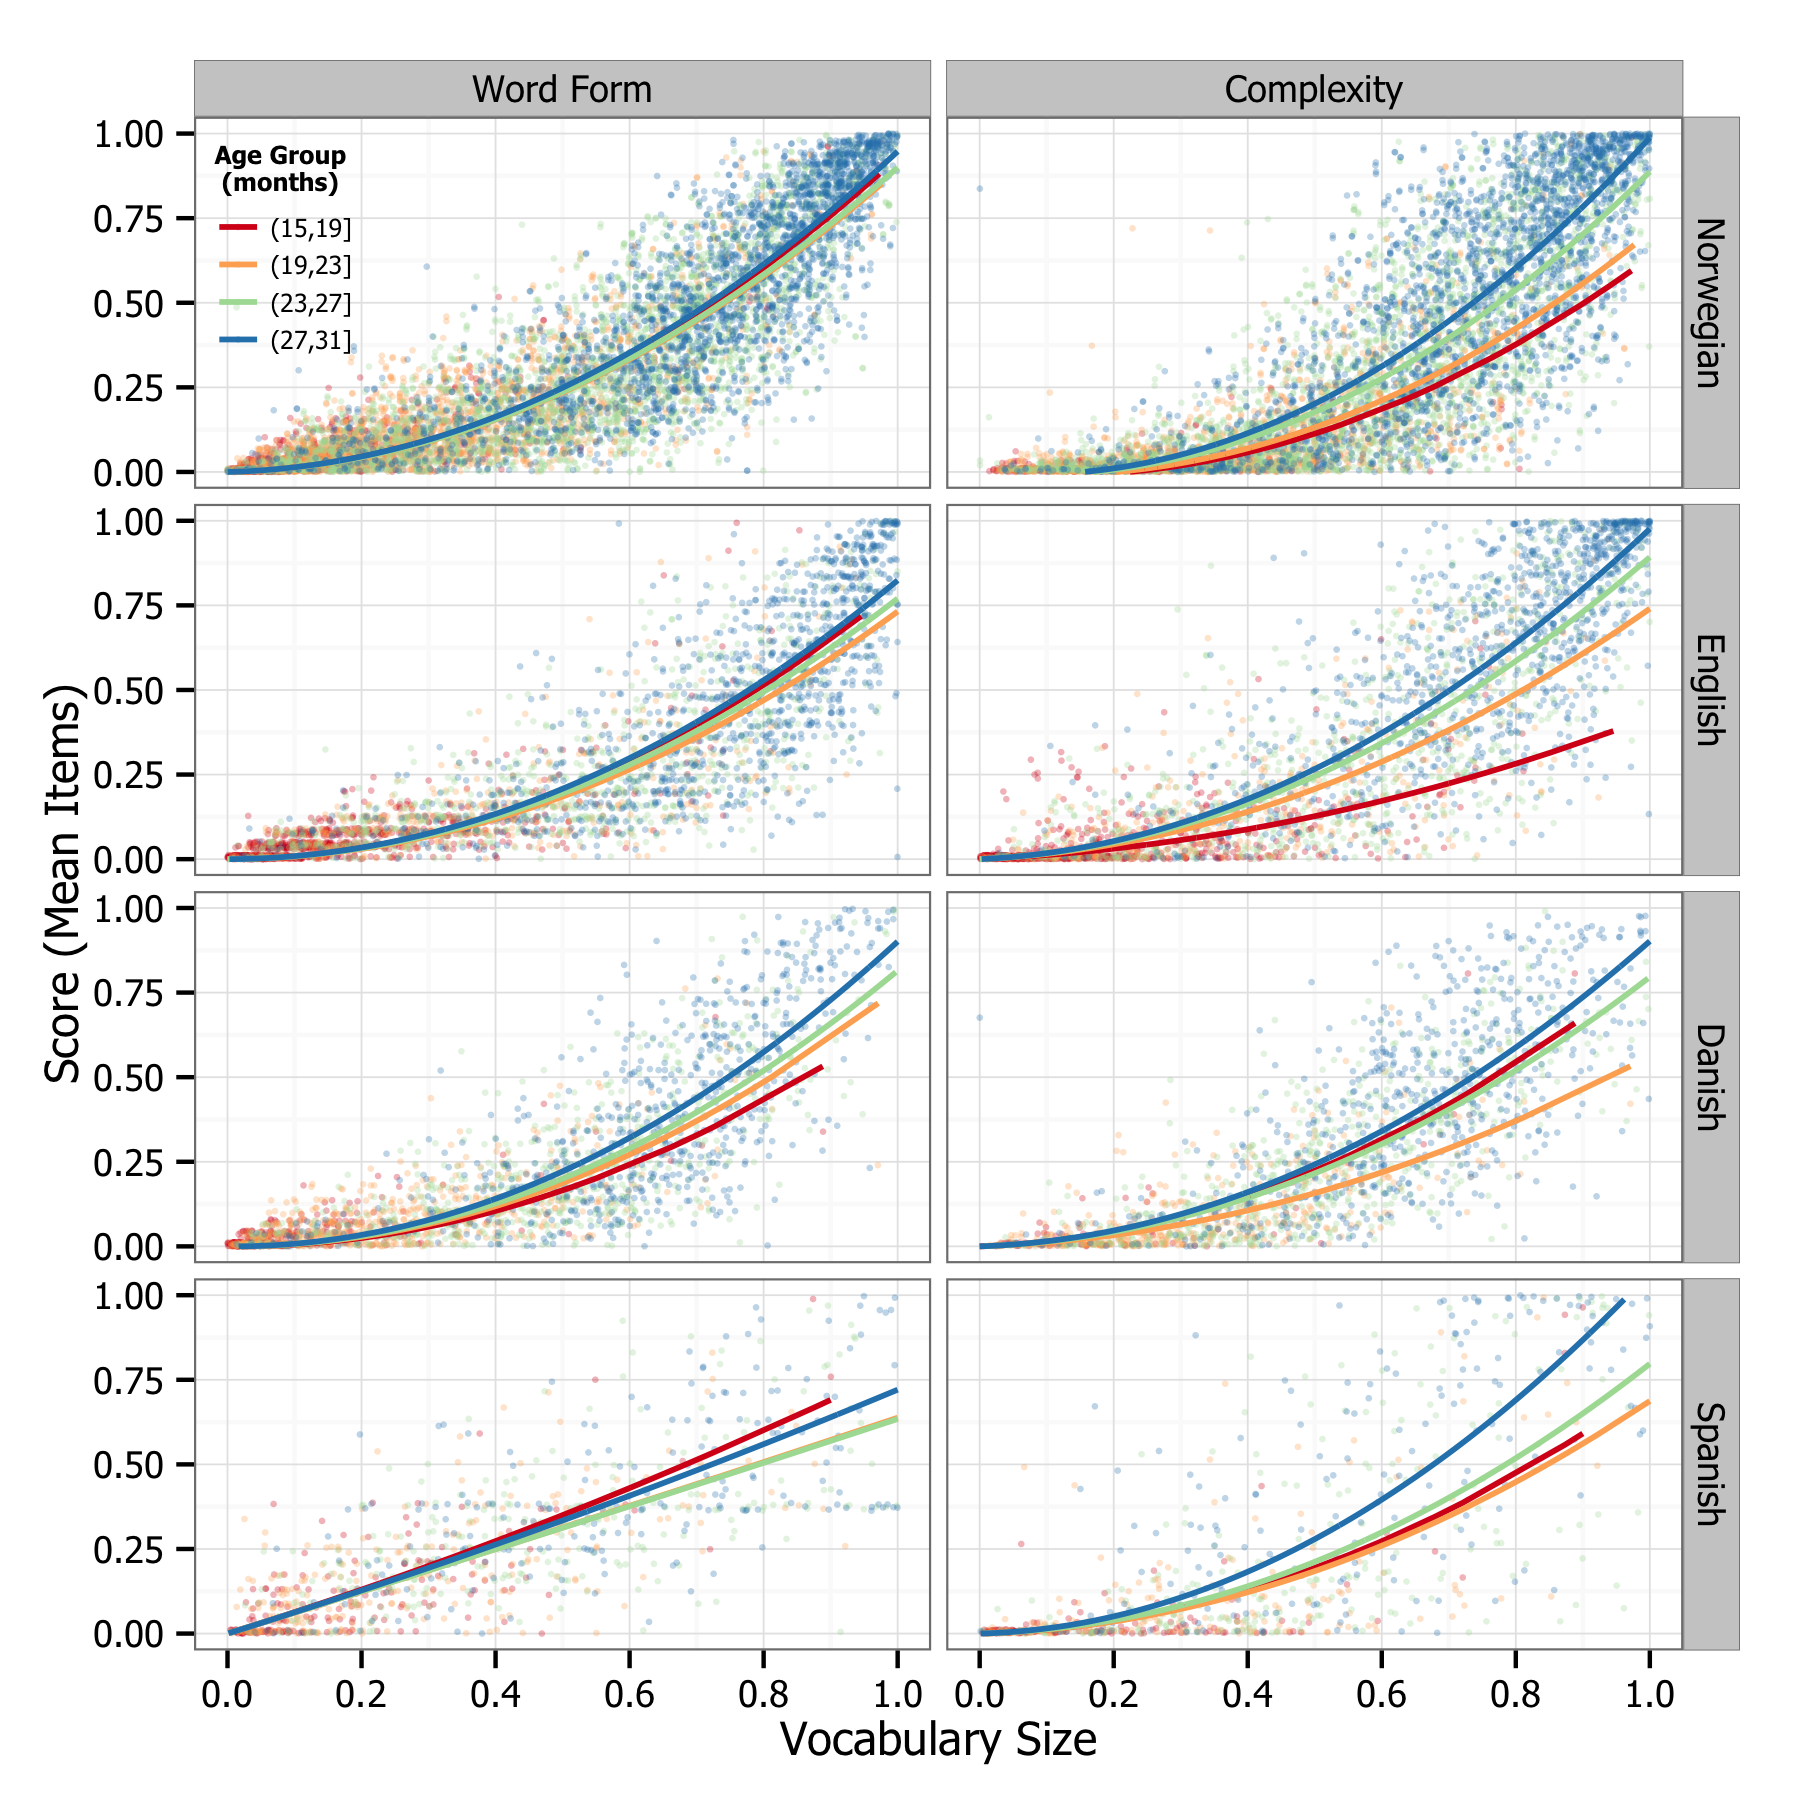
\includegraphics[width=.75\textwidth]{plots/grammar.png}
\caption{\label{fig:grammar} Each point shows an individual child, indicating their total vocabulary size and word form score or complexity score, with color showing their age bin (English $n=4137$; Spanish $n=1094$; Norwegian $n=8505$; Danish $n=2074$). Panels show different languages, and curves are regression models fit separately for each language and measure. The models were specified as \small{\tt{score $\sim$ vocab + age}}.} 
\end{figure*}

By two years, most children have a sizable working vocabulary, including verbs, prepositions and closed class forms that perform grammatical work. They are also beginning to use two- or three-word combinations (e.g., ``mommy sock'') and may demonstrate productive use of inflectional morphemes (e.g., past tense ``-ed''). Previous studies have found a strong connection between the size of the lexicon and grammatical development, as measured by the complexity section, in a variety of languages, including English, Italian, Hebrew, and Spanish \cite<see>{bates1999}. However, no studies have had the power and cross-linguistic representation to go beyond this initial finding. We extend it by examining grammatical development using two different measures: the word forms checklist as a window into morphology and the complexity checklist as a window into syntax. For each measure, we investigate the interaction of vocabulary size and age in a variety of languages.

%This suggests that the mechanisms guiding vocabulary and grammar learning are highly interdependent \cite{tomasello2003,bresnan2001}, a view at odds with the nativist assumption that grammar emerges independent of the lexicon \cite{chomsky1981}.

\subsubsection{Results}

\begin{figure}
\begin{center}
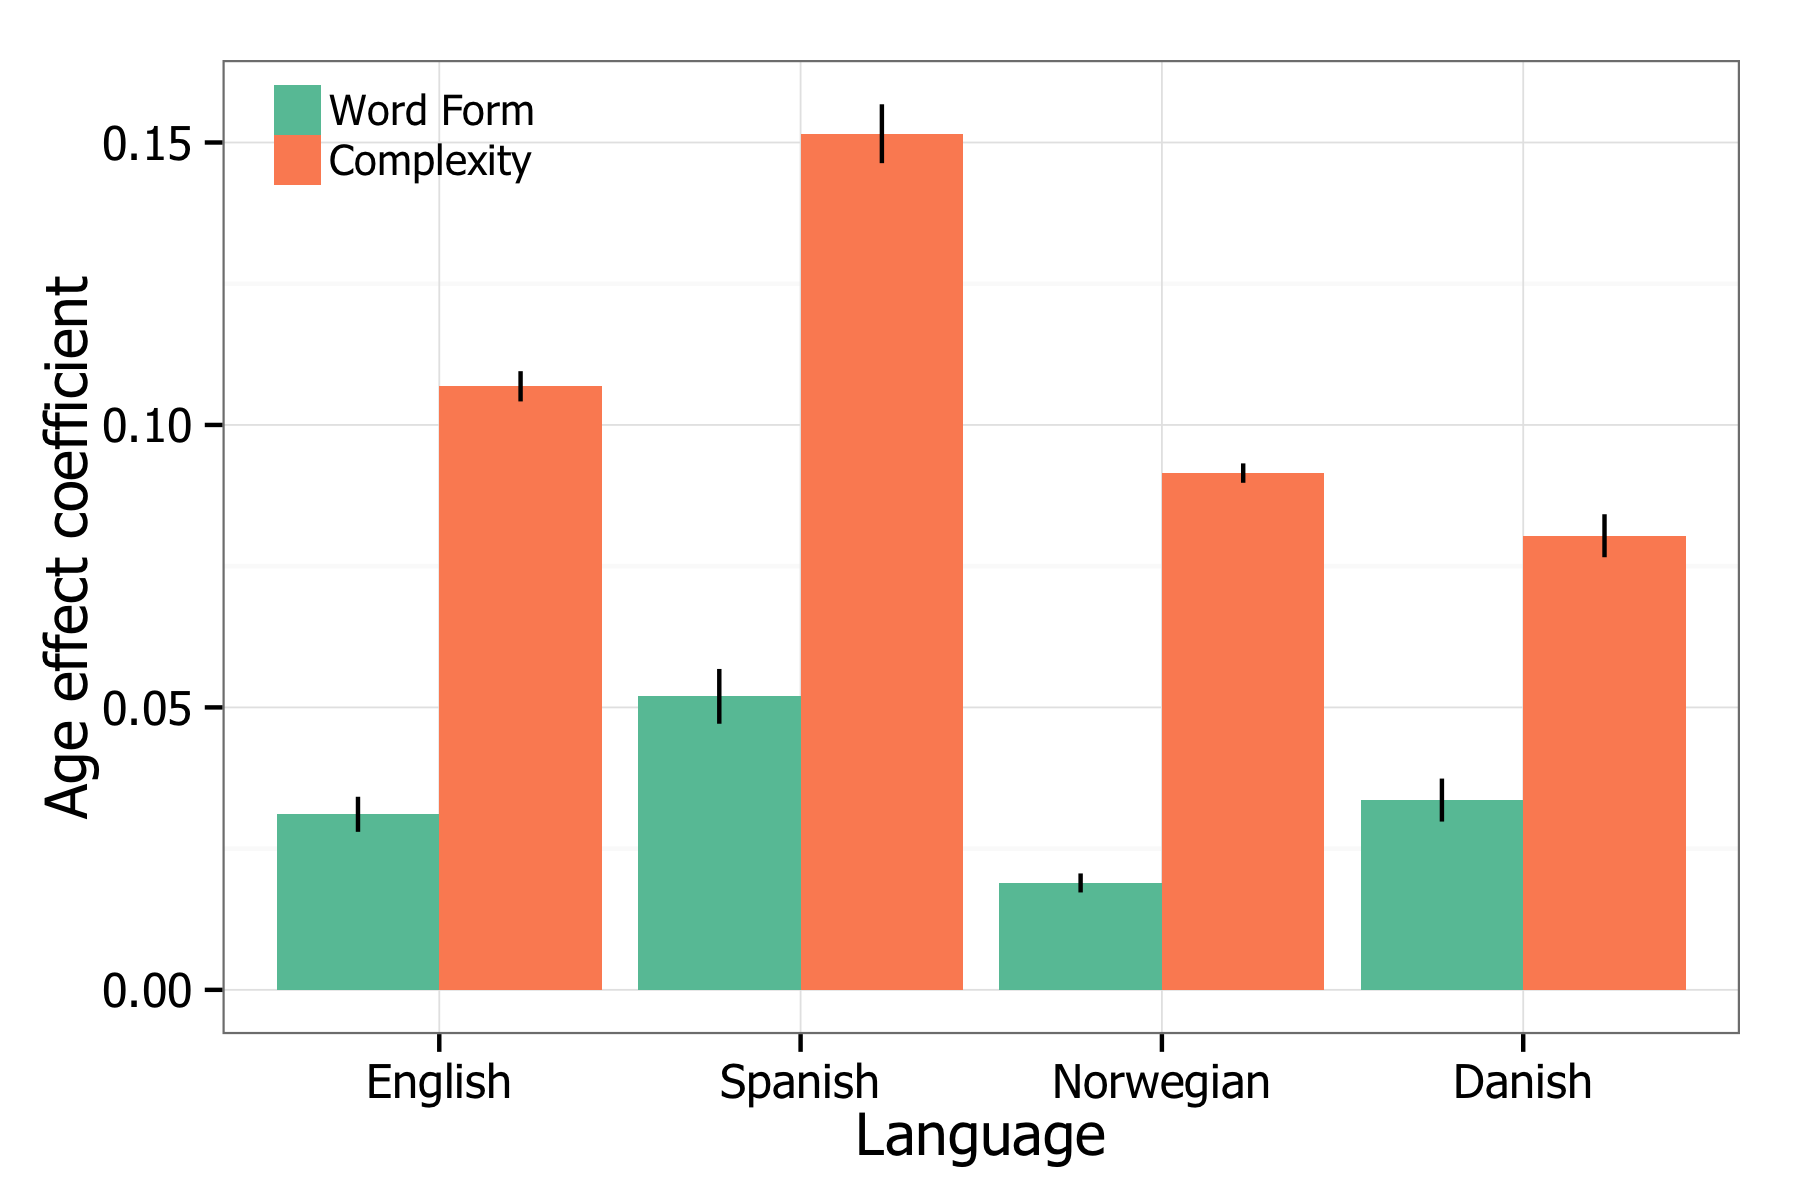
\includegraphics[width=\linewidth]{plots/coefs_wordform_complexity.png}
\end{center}
\caption{\label{fig:coefs_grammar}  For each language and measure (word form and complexity), the coefficient of the interaction between vocabulary size and age. Error bars show the standard error of the coefficient estimate. Across languages, complexity has a substantially larger interaction with age effect than word form, suggesting that age contributes more additional variance beyond vocabulary size for measures of grammar that are based on syntax than morphology.} 
\end{figure}

For each language, we wanted to estimate how much variance in children's syntactic and morphological development remained after knowing that child's vocabulary size. Specifically, we asked whether age provided additional predictive power over and above vocabulary size. To estimate this effect, we fit logistic regression models to each child's word-form and complexity scores. We modeled each child's score as a function of vocabulary size and age in months. Main effects were always exceedingly reliable, but the interaction term had negligible magnitude and so we omit it here. Figure~\ref{fig:grammar} shows data and models. Each dot represents an individual child's score on each measure, while curves show the relationship between that measure and vocabulary size. 

\begin{figure*}
\centering
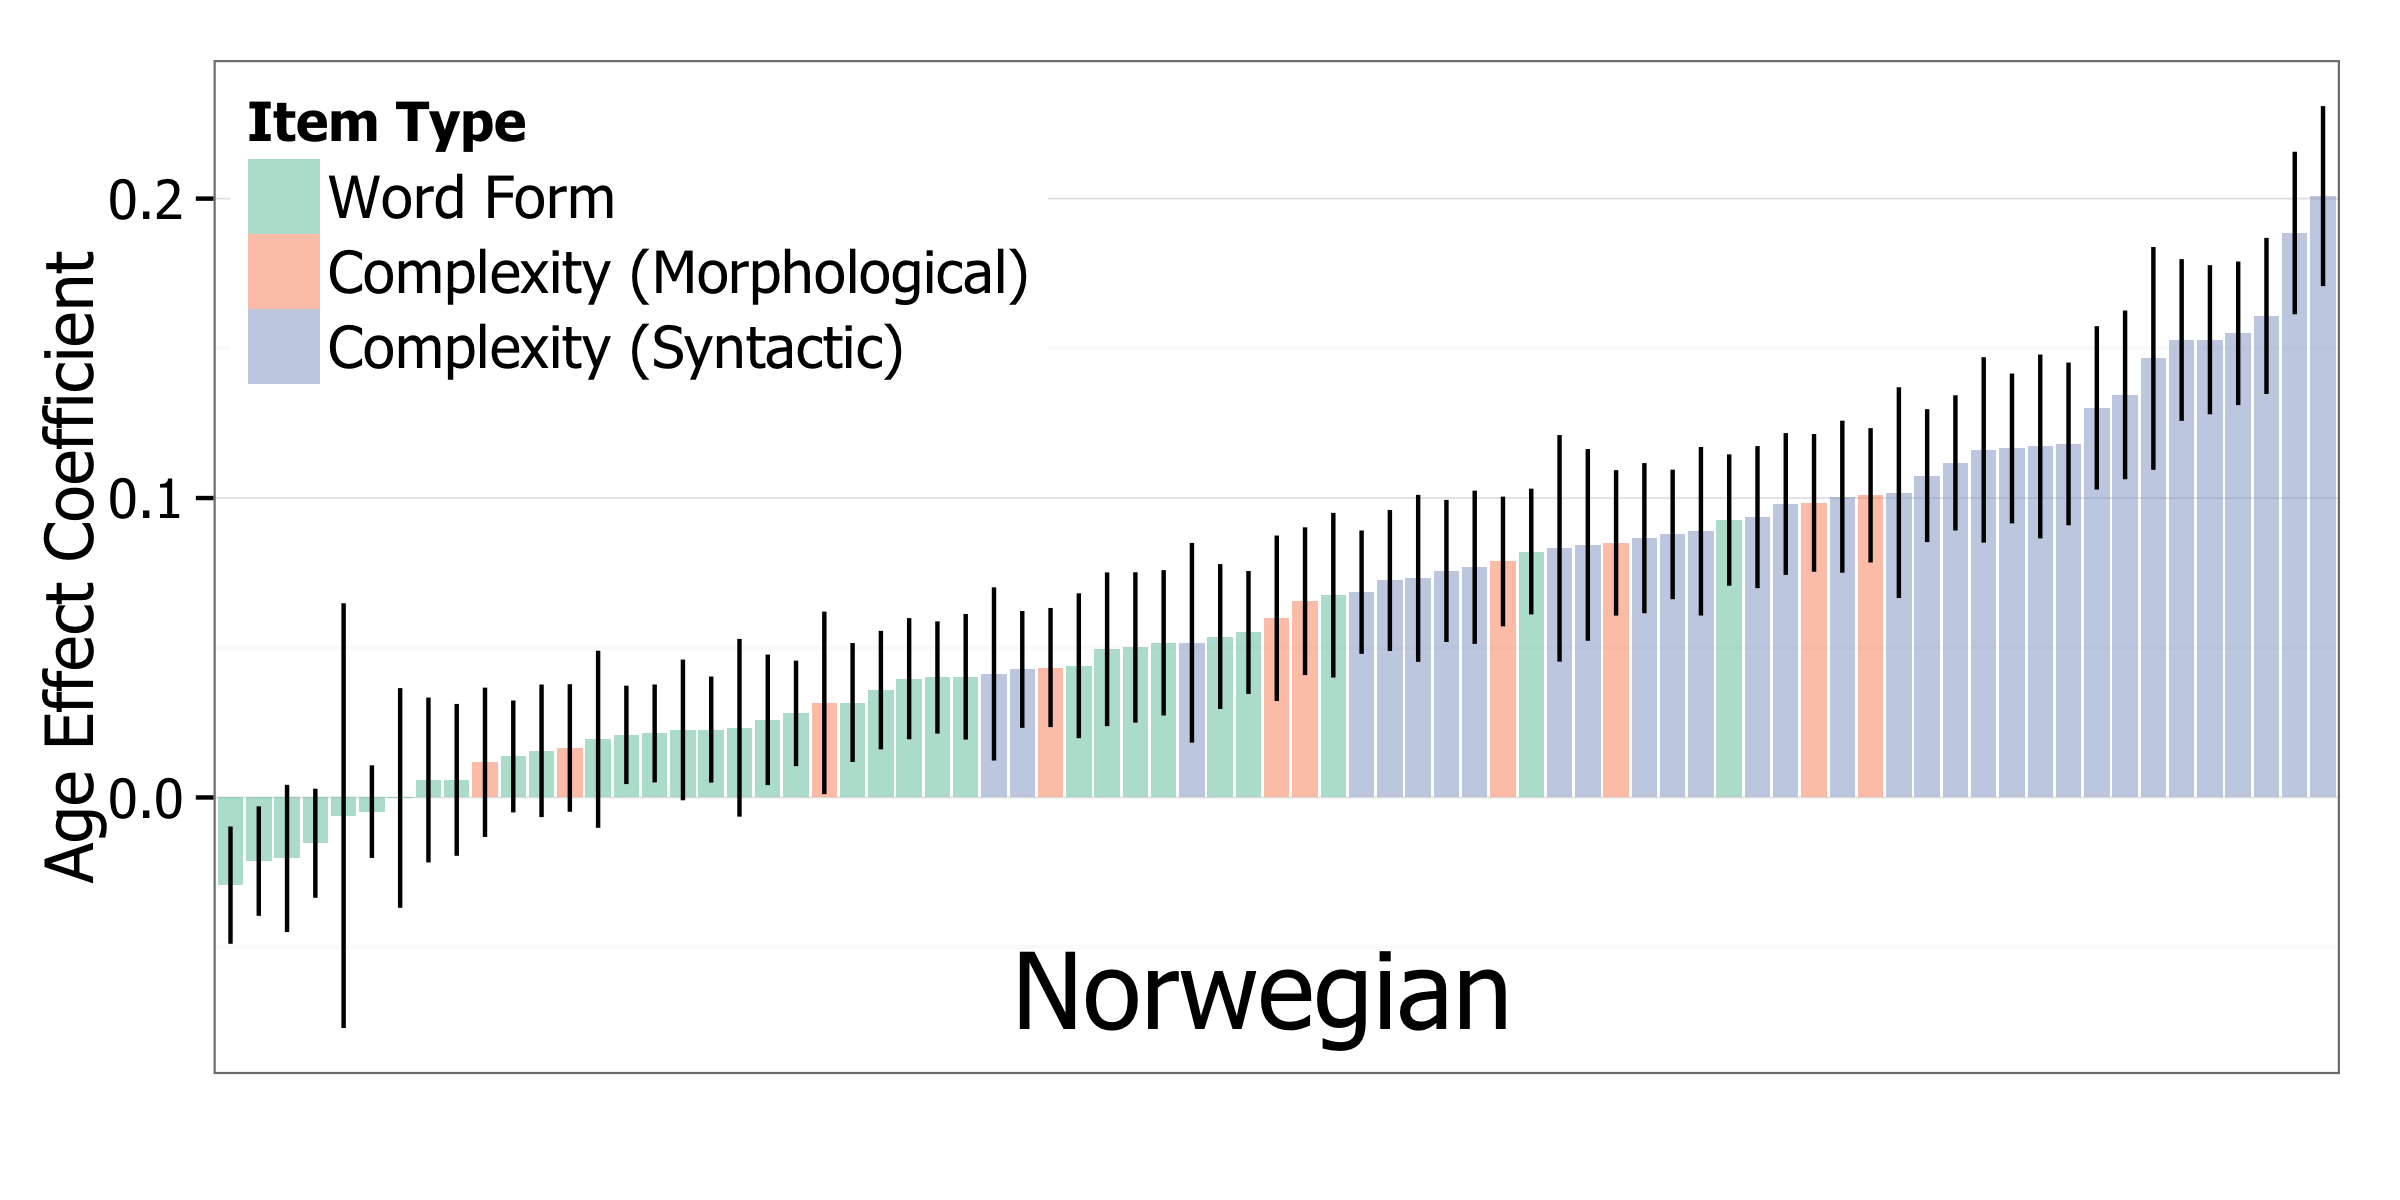
\includegraphics[width=.49\textwidth]{plots/norwegian_interactions}
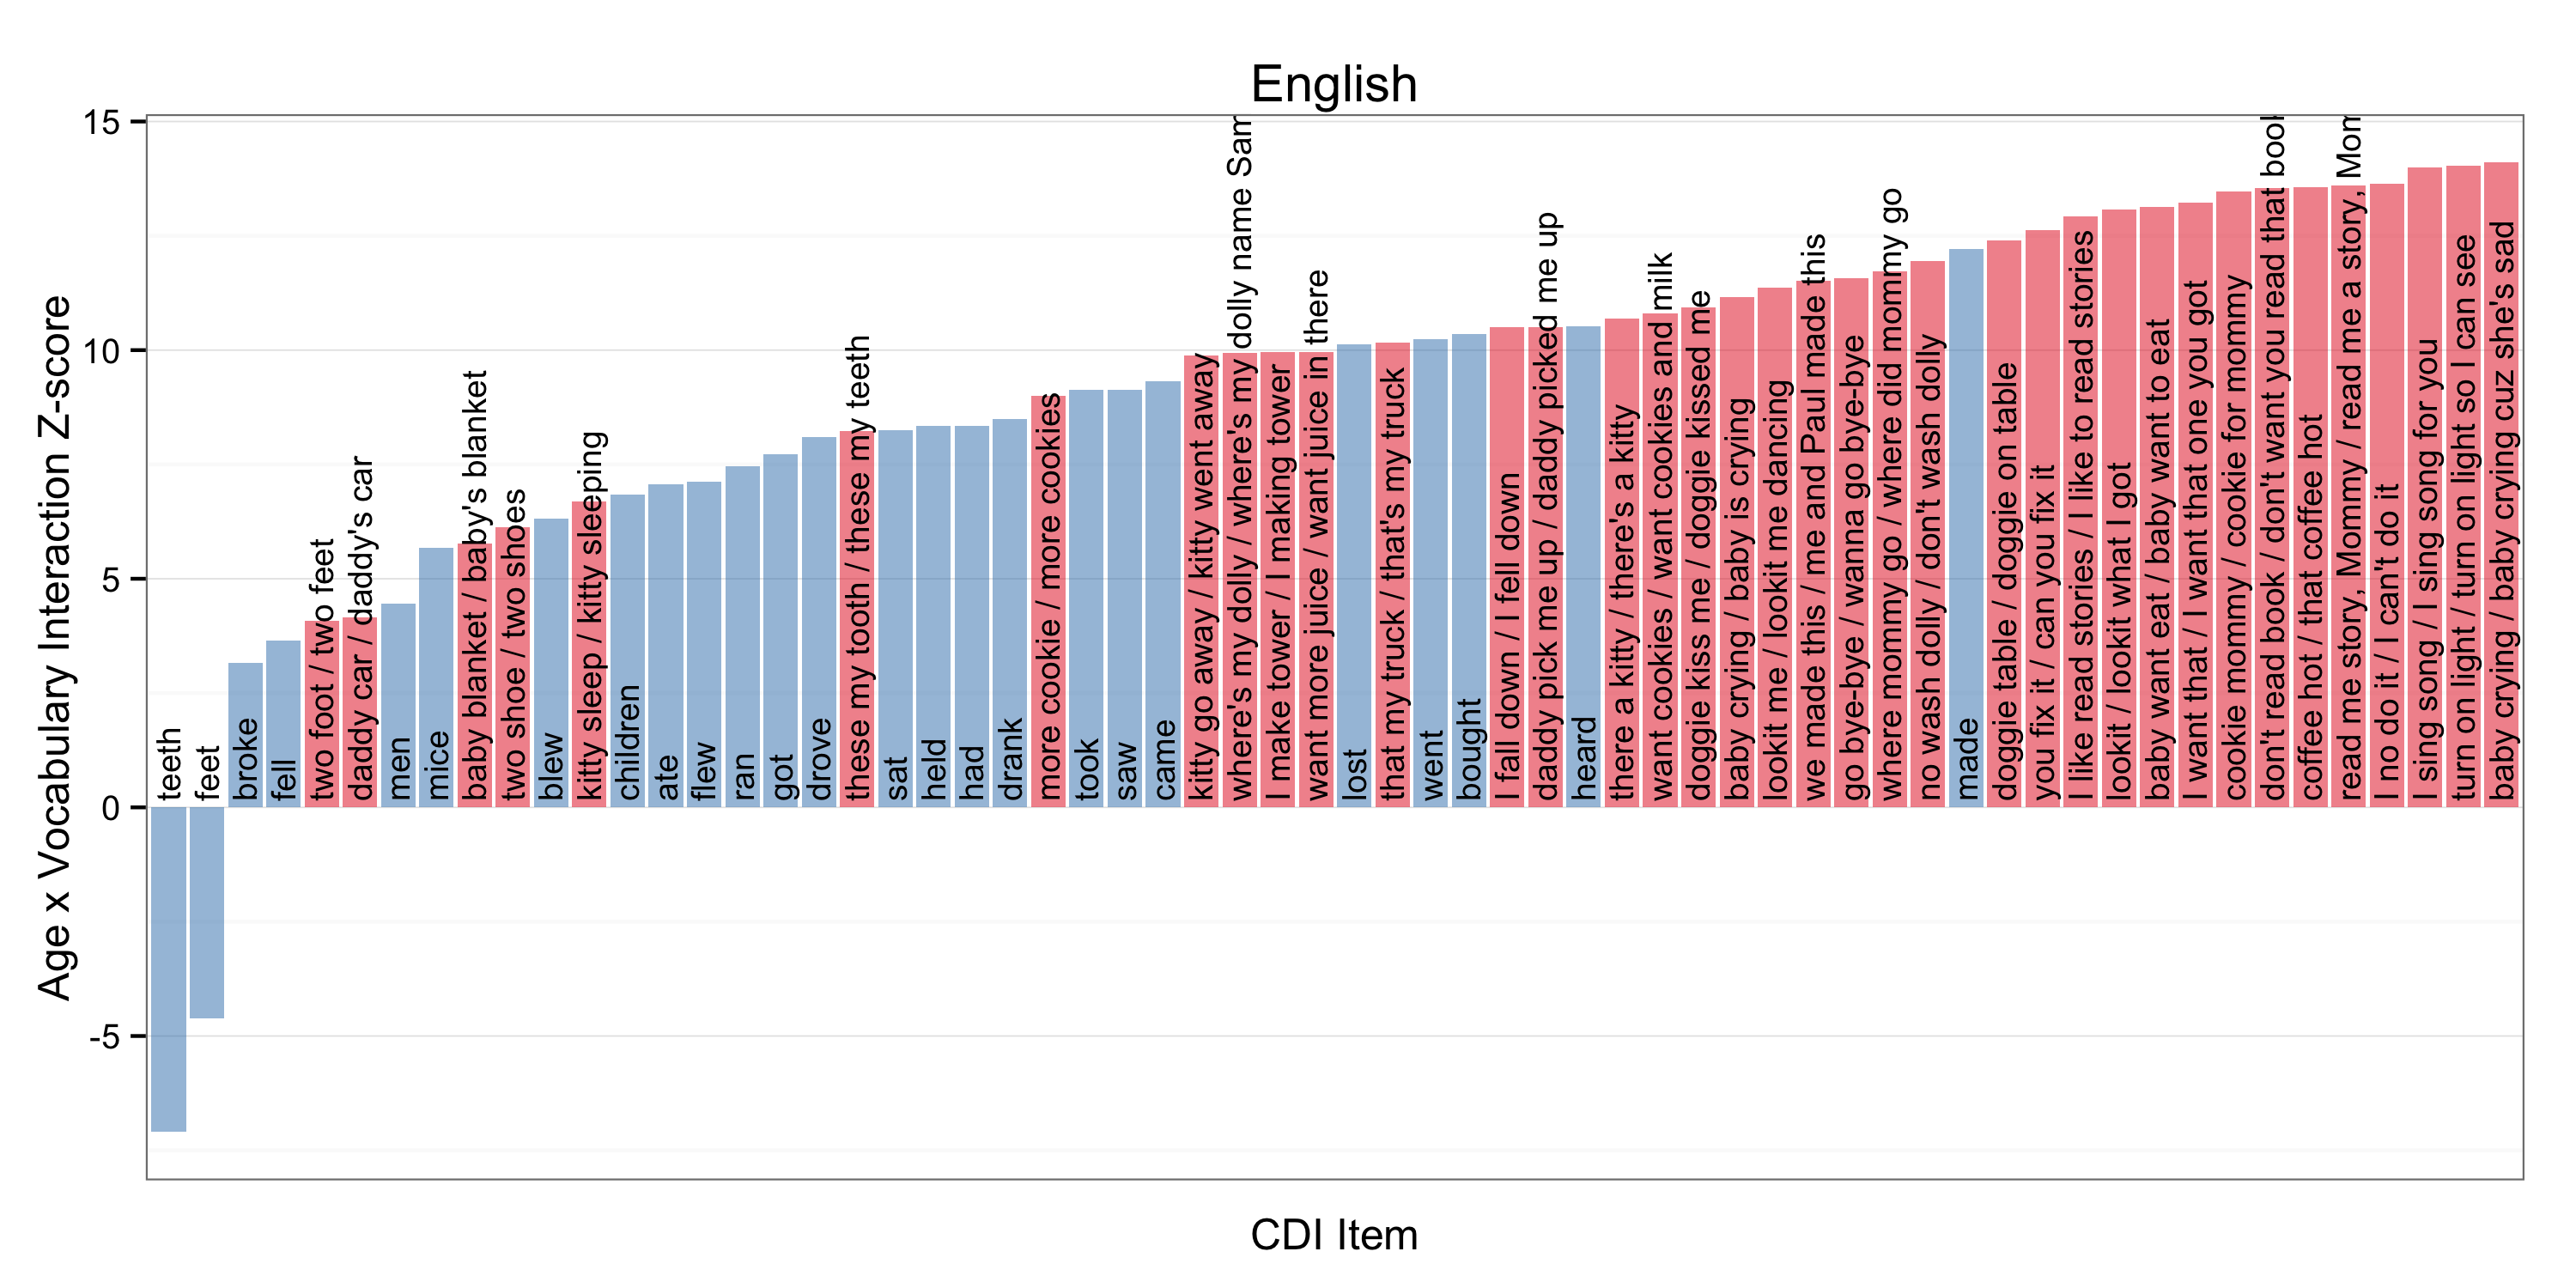
\includegraphics[width=.49\textwidth]{plots/english_interactions}\\
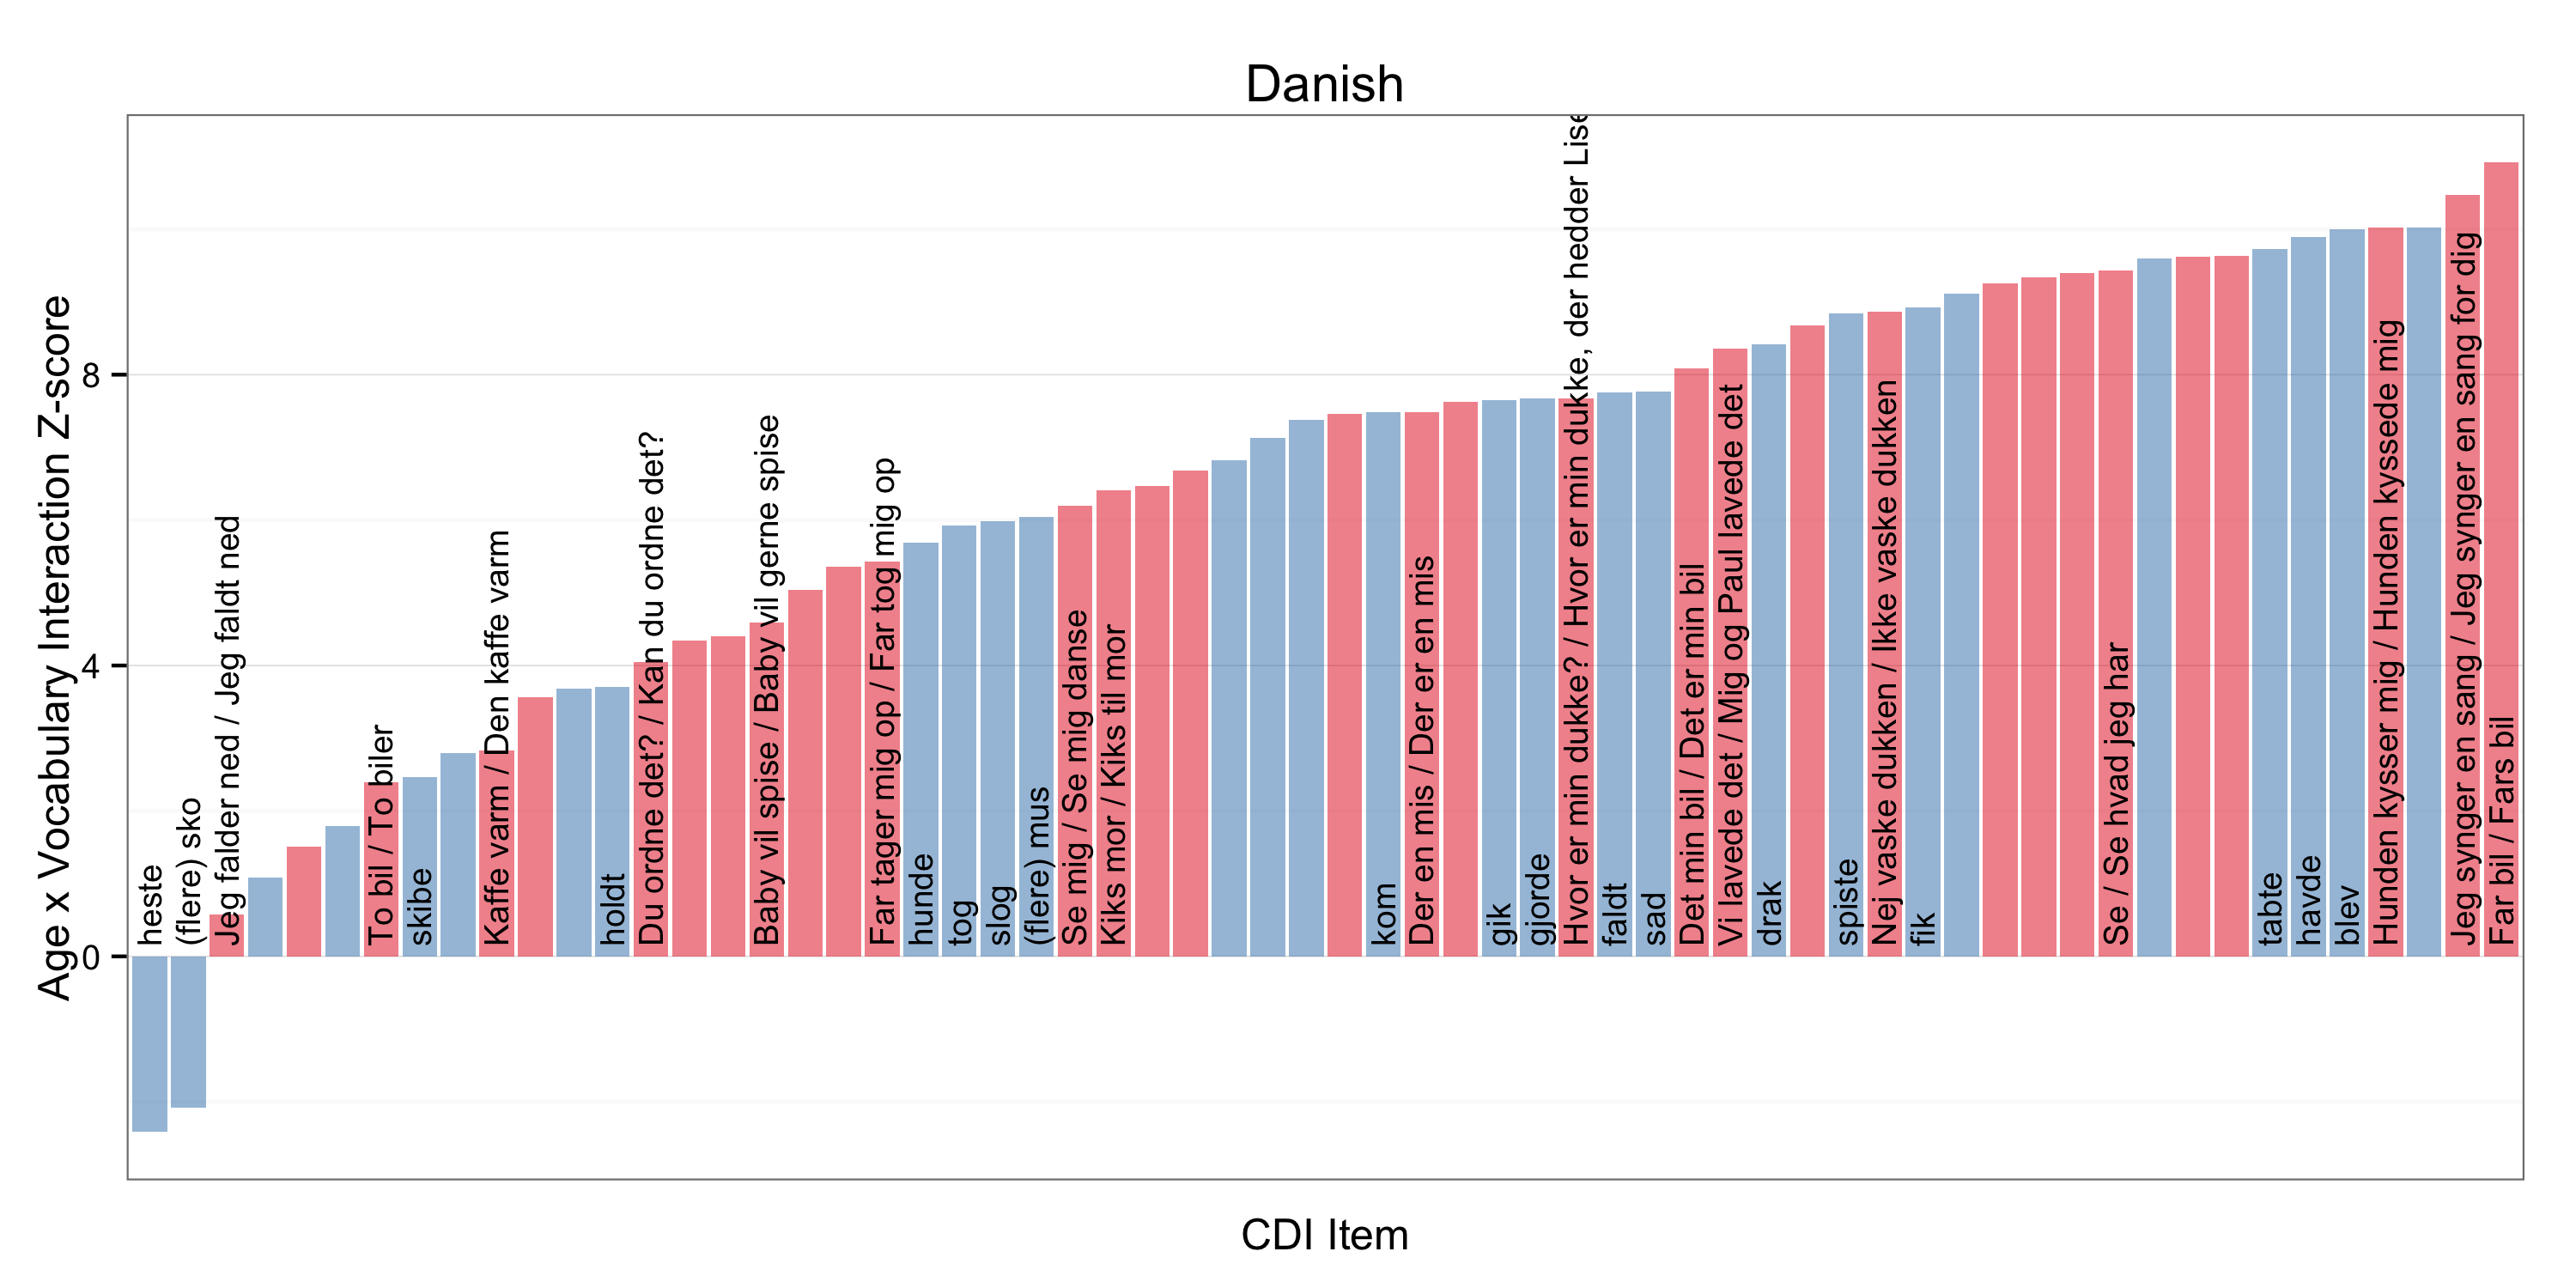
\includegraphics[width=.49\textwidth]{plots/danish_interactions}
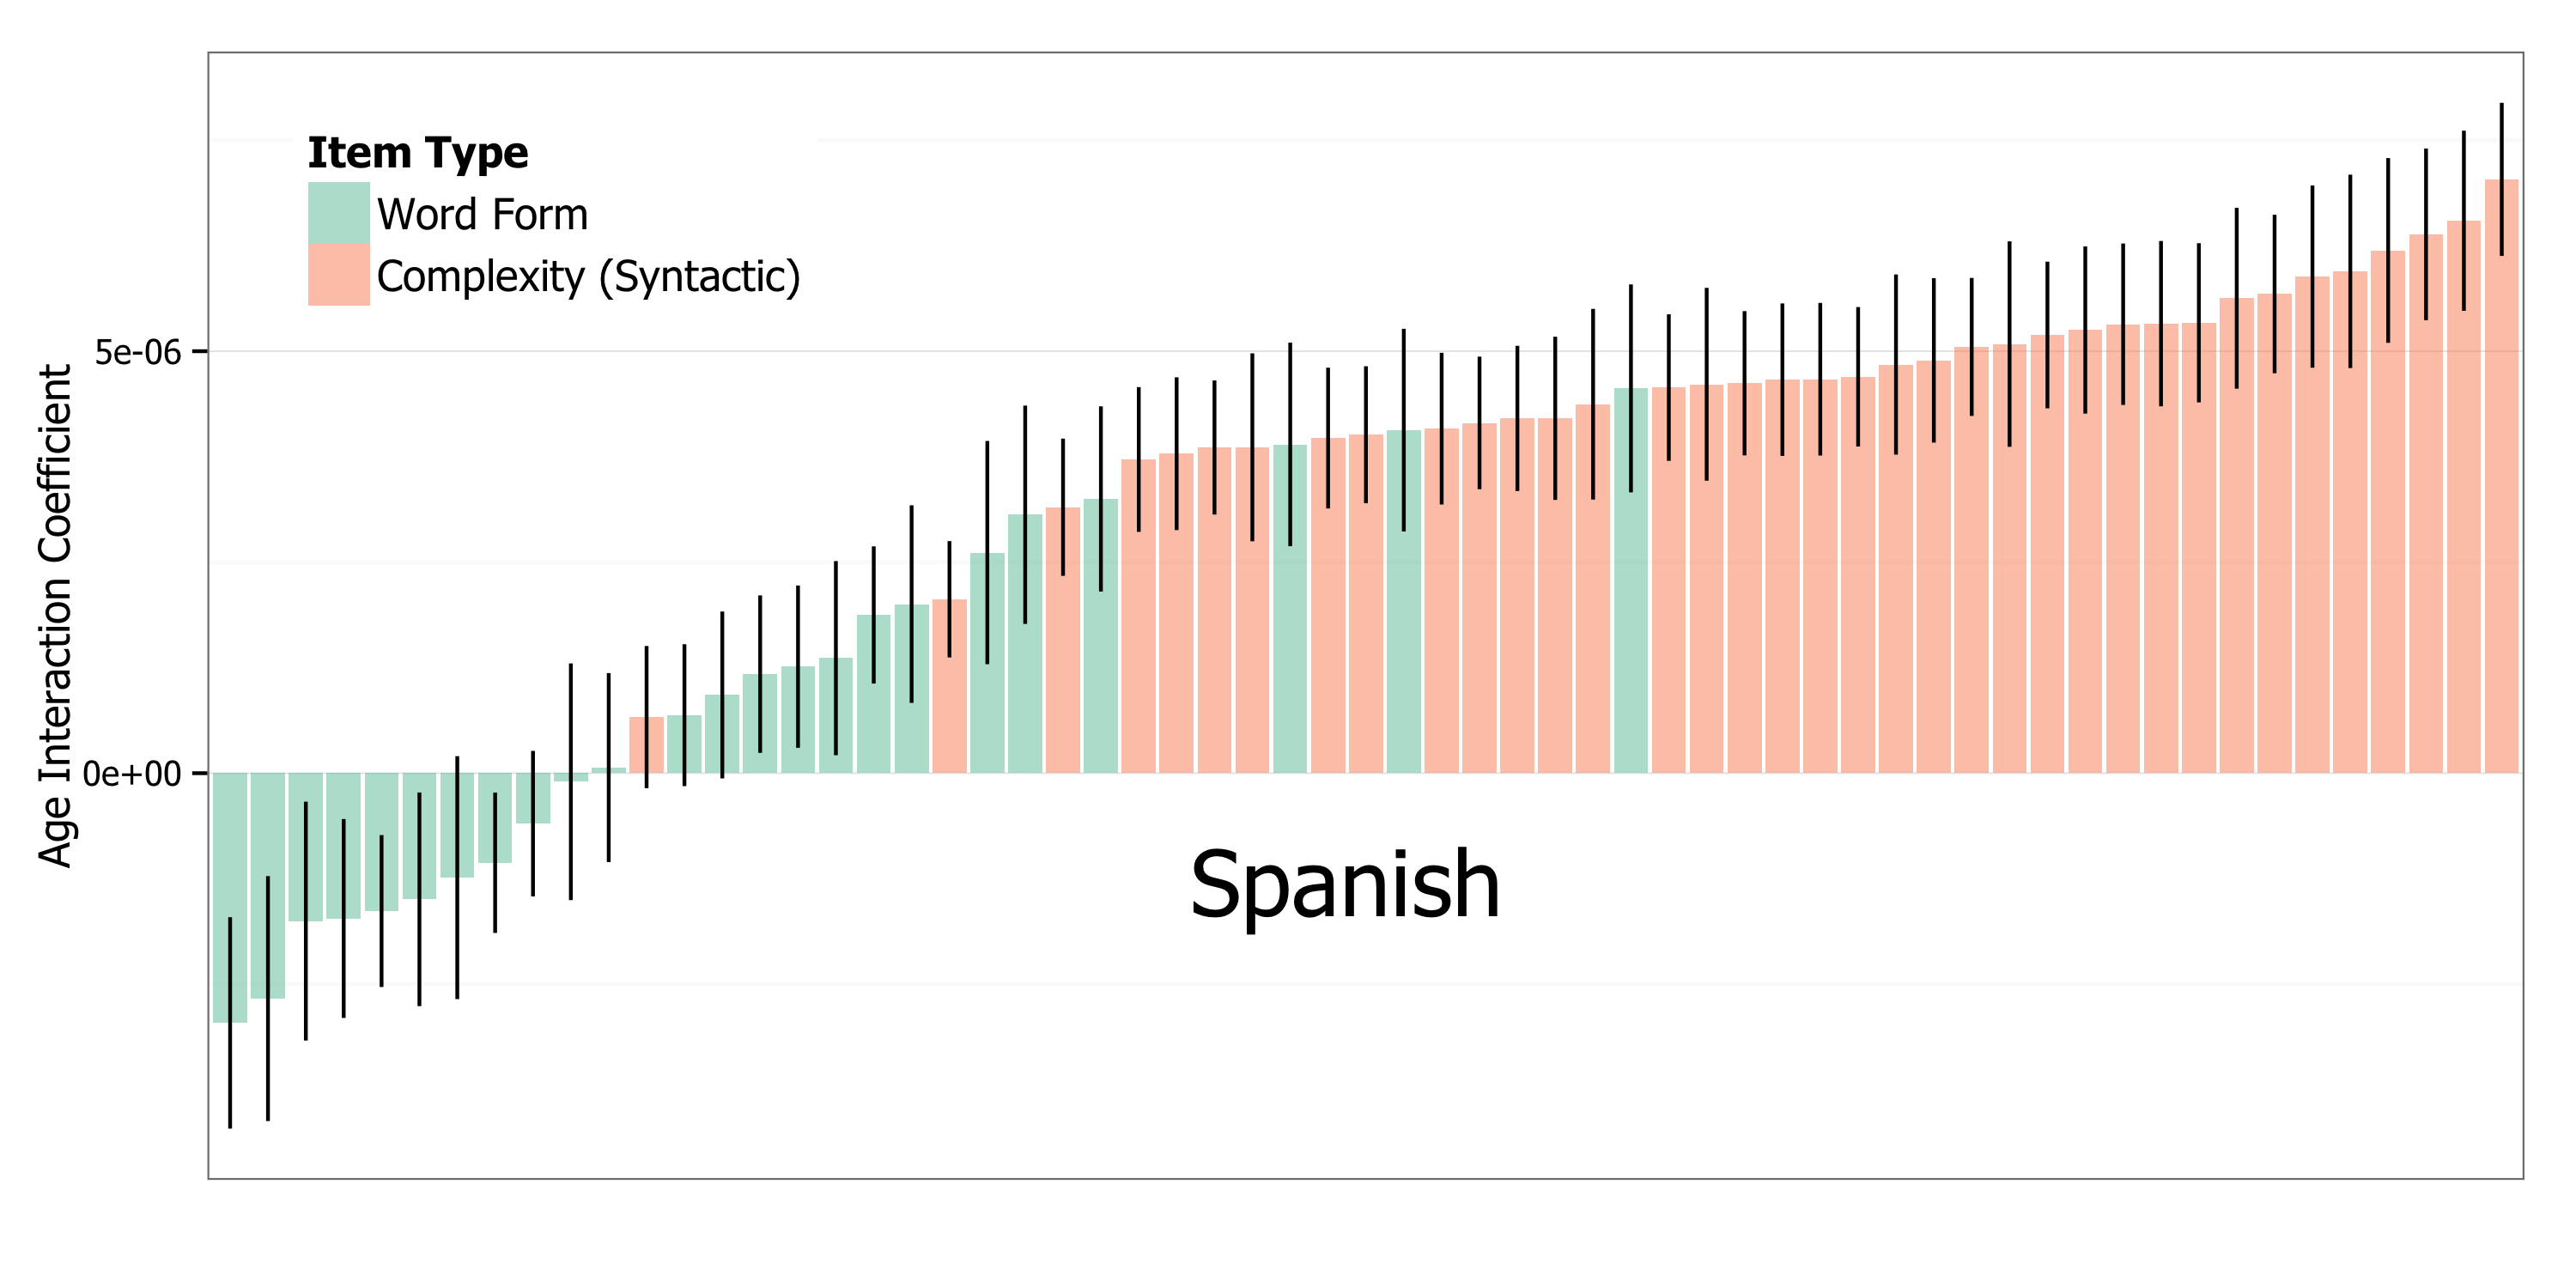
\includegraphics[width=.49\textwidth]{plots/spanish_interactions} 
\caption{\label{fig:interactions} For each language and item, the z-score of the model's age effect. Across languages, complexity items tend to have a substantially larger age effect than word form items. No Spanish complexity items had exclusively morphological content.}
\end{figure*}

As seen most clearly for English and Norwegian---the languages for which we have most data---the curves on the left-hand panel are virtually overlapping, showing little differentiation across the age groups.  This indicates only small additional contributions of age above and beyond vocabulary.  In contrast, the curves in the right hand panel for the complexity items show a characteristic fan across each of the age groups.  This indicates that the relationship between vocabulary size and complexity score is modulated by age. The Spanish and Danish data show less of a clear complexity curve fan, possibly because of the relatively small number of data points in the youngest age group.

Because of the size of our samples, all main effects and interactions were highly significant in each language. To assess the extent of the age contributions to children's morphological than syntactic development, we compared the coefficients in our models across languages and measures. Figure~\ref{fig:coefs_grammar} shows the interaction between age and vocabulary size for each of these models across languages. In each model, the age-related interaction coefficient is substantially larger for the complexity sections than for the word form sections, indicating a greater developmental effect on those items that generally align with syntax than inflectional morphology.  

Given the heterogeneous nature of the CDI instruments, particularly of the complexity sections, we further break down the items of the complexity sections by classifying them as capturing more morphological or more syntactic phenomena. We then fit predictive models as above, but separately for each word form and complexity item. Figure \ref{fig:interactions} shows the coeffcients of the age-interaction terms of the models for each item. In general, there is a clear three-way split: age effects are smallest for Word Form items, then morphological Complexity items, and largest for syntactic Complexity items, again supporting the hypothesis of greater age-contributions to relatively more syntactic phenomena. 

\subsubsection{Discussion}

Building on previous analyses that showed a strong relationship between lexical and grammatical development, we added age into this relationship. Our measures of syntactic development consistently showed greater age modulation than morphological development across languages. Further distinguishing between items that were more reflective of morphology compared with syntax, we again found greater age effects for more syntactic items.  Thus, this analysis provides evidence for the relationship between syntactic development and age, over and above the variance associated with lexical development. 


\subsection{Analysis 2: Vocabulary Composition}


Early vocabulary development is typically characterized by learning of names for caregivers and common objects, while later in development, children tend to increase their vocabulary by increasing the proportion of predicates (verbs and adjectives). This over-representation of nouns has been found across a number of analyses and in a variety of languages \cite{bates1994,caselli1995,bornstein2004}, though not all \cite{tardif1996,choi1995}.
%\footnote{Differences in early vocabulary composition have been argued to emerge from typological differences (e.g., word order, subject drop), and from cultural practices (e.g., focus on picture book reading) \cite{tardif1999, gopnik1996, choi1995}---we are agnostic as to the source of this variability.}
For our purposes we are interested in using these analyses of vocabulary composition to test for the same kind of age-related differences that we found in the complexity and word-form analyses. 

\begin{figure*}
\begin{center}
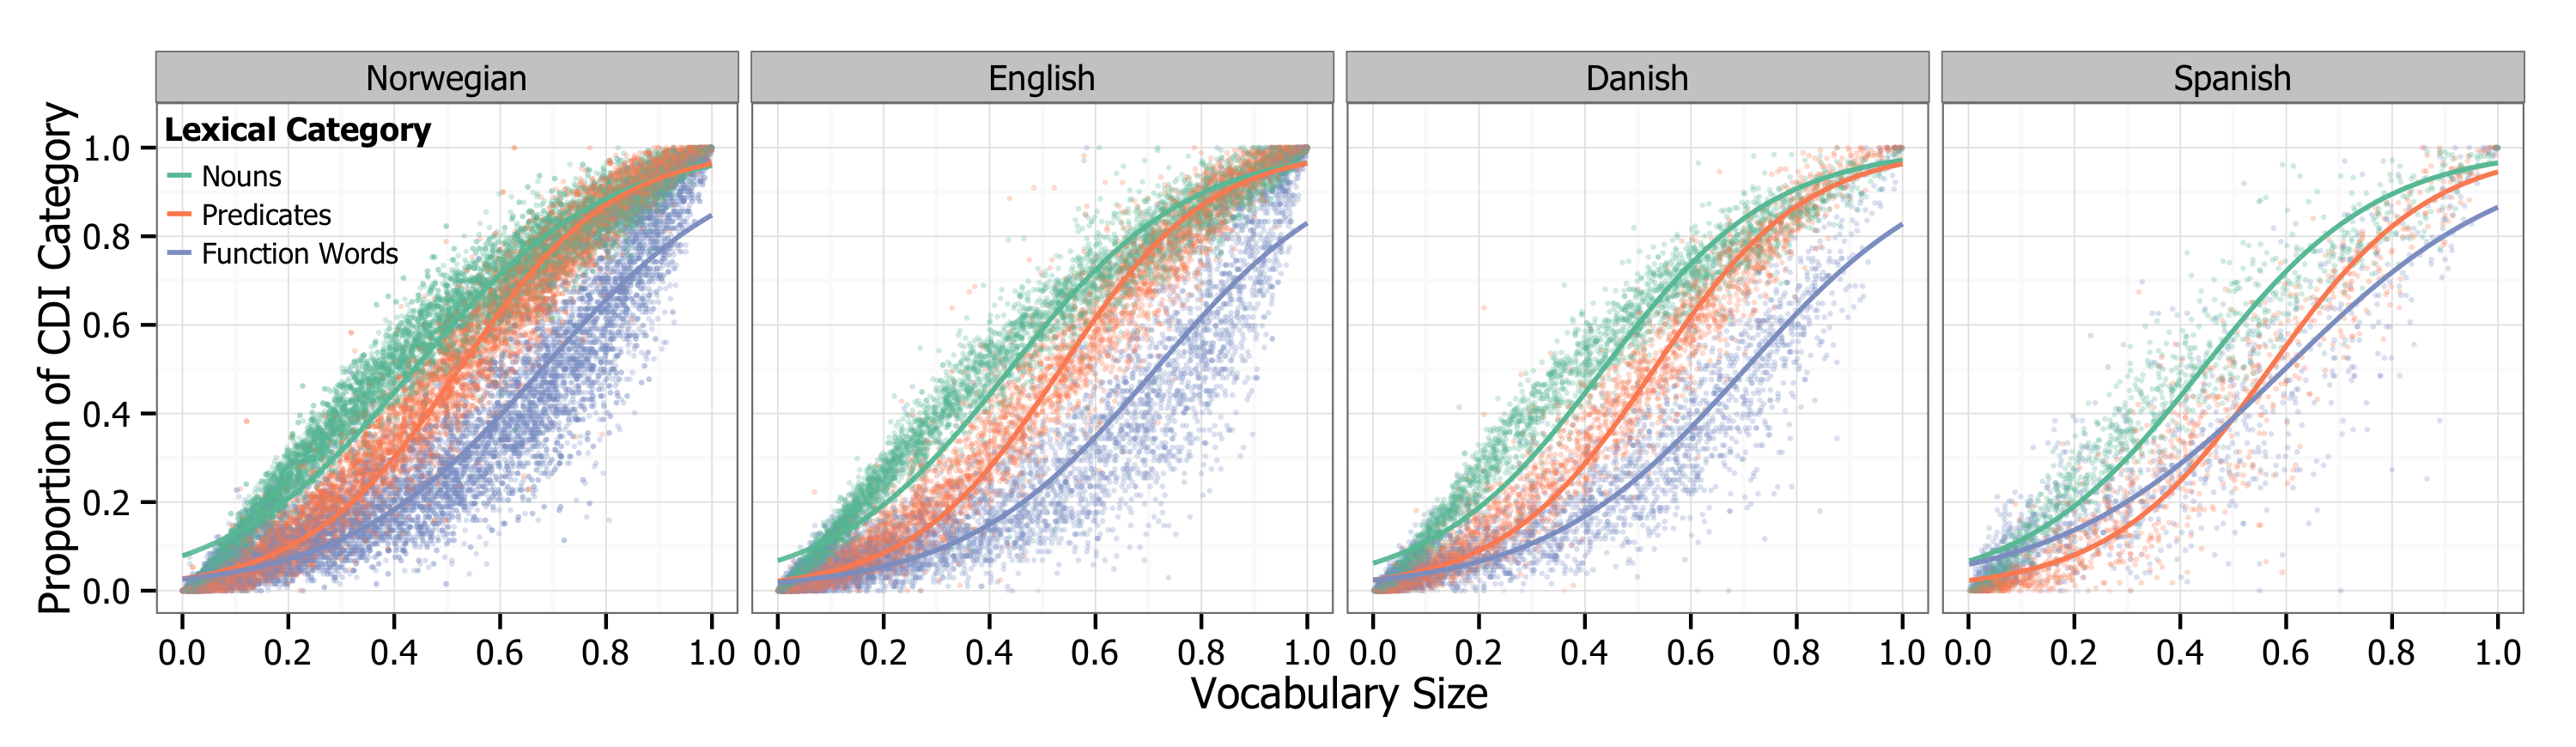
\includegraphics[width=\textwidth]{plots/composition_fit.png}
\end{center}
\caption{\label{fig:vocab_comp} Proportion of a particular CDI category, plotted by total vocabulary size. Each point shows an individual child, with color showing their noun, predicate, and function word vocabulary. Panels show different languages, and curves are smoothing functions using loess (English $n=5595$; Spanish $n=1094$; Norwegian $n=10095$; Danish $n=3038$).} 
\end{figure*}

We predict that the proportion of predicates (verbs, adjectives, adverbs) in children's vocabulary should be relatively more affected by age than nouns. Concrete nouns are hypothesized to be learned initially from both co-occurrences between words \cite{yu2007b} and by social cues to reference to particular objects \cite{bloom2002}. On neither of these accounts should syntactic information be a primary information source (though of course syntax might be more informative for abstract nouns). In contrast, for verbs, syntax has been argued to be crucial for learning. On the syntactic bootstrapping hypothesis \cite{gleitman1990,fisher2010}, verbs especially are learned by mapping the syntactic structure of utterances to the thematic structure of observed events, for example by noticing that the subject of a sentence matches the agent in one particular ongoing event but not another (``the cat is fleeing the dog'' matches {\sc flees(cat, dog)} but not {\sc chases(dog,cat)}). At a high level of description, a similar argument can be made for adjectives, where identification of the modified noun is similarly critical. Thus, if syntactic development is related in some way to age, we should see larger age effects on predicate vocabulary than noun vocabulary. 

\subsubsection{Results}

Each CDI form contains a mixture of words in different classes. We adopt the categorization of \citeA{bates1994}, who split words in nouns, predicates (adjectives, adverbs, and verbs), function words, and other words. Then, for each child's vocabulary, we compute the proportion of the total words in each of these categories that they are reported to produce. This yields a set of proportions for each child.

For each of the four languages in our sample, we plot these proportions against total vocabulary. These functions are shown in Figure \ref{fig:vocab_comp}: Each dot represents an individual child's knowledge of a particular class, while curves show the relationship between that class and the entirety of the vocabulary. If categories grow independently of one another, these curves should approximate the diagonal. This pattern is not what either we or \citeauthor{bates1994} observed however: Across the languages in our sample, nouns are systematically over-represented in smaller vocabularies (shown by a curve that is above the diagonal), while function words---and to some extent, predicates---are under-represented. 

Next, we measure the contribution of age to vocabulary composition. We fit a logistic model to all children's data for each word class, predicting word-class proportion as a function of total vocabulary and age (as in Analysis \#1). Figure \ref{fig:coefs_noun_verb} shows age coefficients for each of these models across languages. In each model, the age-related interaction coefficient is substantially larger for predicates (and for function words) than for nouns. This asymmetry can be interpreted as evidence that for two vocabulary-matched children, the older would tend to have relatively more predicates and function words than the younger.

\subsubsection{Discussion}

We replicated previous analyses \cite{bates1994} showing an over-representation of nouns in the developing lexicon and a relative under-representation of predicates. We also predicted that---if syntactic generalization was in some way tied to age---predicates and function words would show relatively more age influence than nouns. This prediction was confirmed across all four languages we examined. Thus, this analysis provides additional circumstantial evidence for a relationship between syntactic development and age, independent of the growth of the lexicon.

\begin{figure}
\centering
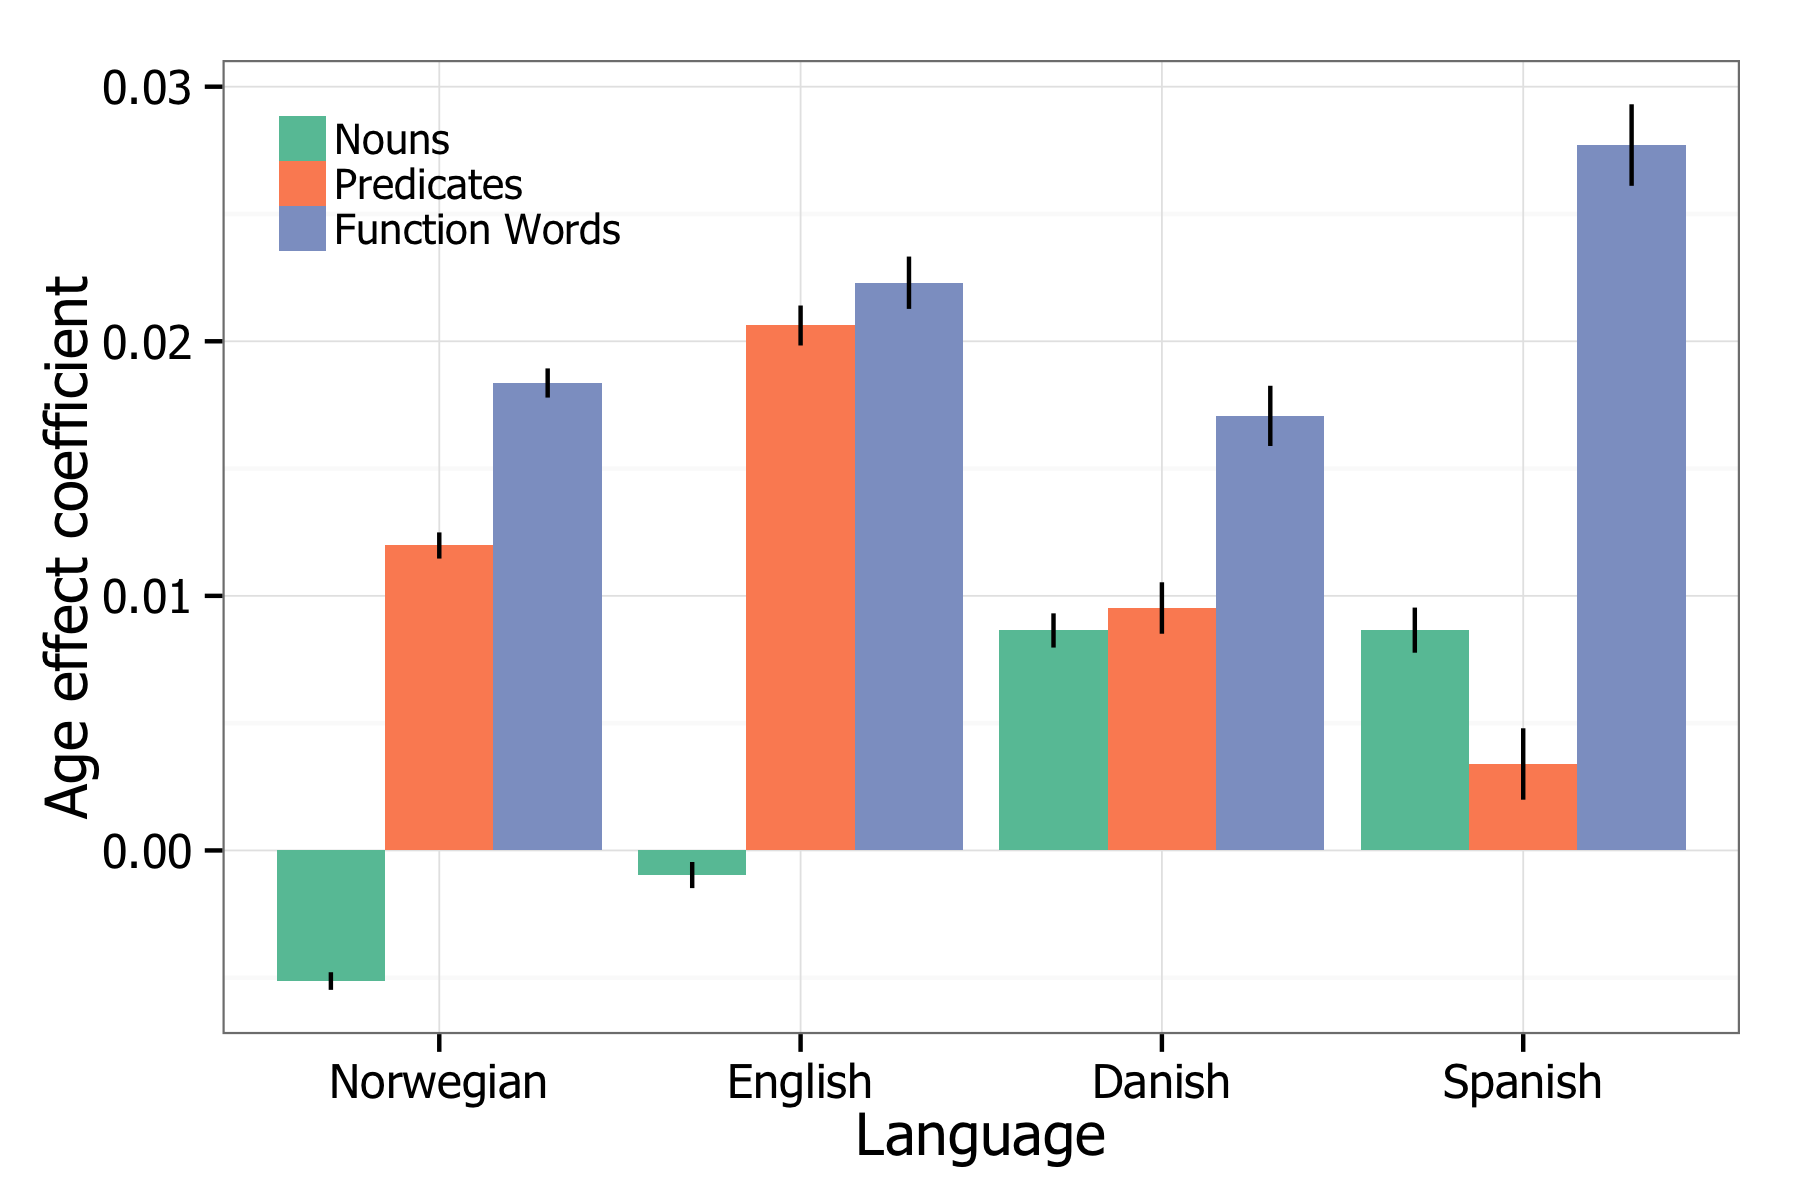
\includegraphics[width=\linewidth]{plots/coefs_vocab_comp.png}
\caption{\label{fig:coefs_noun_verb} For each language and lexical category, the coefficient of the model's age and vocabulary size interaction term. Across languages, verbs have a substantially larger age effect than nouns.}
\end{figure}

\section{General Discussion}

The current study addresses novel questions regarding lexical and grammatical development by taking advantage of Wordbank, a newly-developed web-based tool which compiles a large number of CDI forms in many different languages.  Here, we compared estimates of age-related contributions to grammatical development using different approaches: their reported usage of various morphological forms and syntactic constructions, and the substructure of their vocabularies by grammatical category. For each metric, we used vocabulary size as a predictor and examined the interaction of age with this predictive relationship.

Across four languages, we find that measures of grammar that are more closely aligned with syntax are modulated by age to a greater extent than those reflecting inflectional morphology.  Moreover, we find that  developmental changes in verb proportion is modulated by age to a greater extent than noun proportion. Both of these findings suggest a place for developmental processes that facilitate grammatical acquisition, above factors that are reflected in global measures of vocabulary size.

Thus, these analyses suggest interesting new areas of research regarding possible mechanisms driving children's early lexical development and how those mechanisms might support children's transition from single words to more morphosyntactically-complex utterances.  One possibility is that these developmental changes are dependent on maturational factors that operate on grammatical development in a domain-specific way, independent of lexical-semantic processes.  Another possibility is that these age-related effects represent more domain-general learning mechanisms, such as attention or working memory that tend to support sentence-level processes rather than word-internal ones.

% processing speed, working memory? 

\section{Acknowledgments}

Thanks to the MacArthur-Bates CDI Advisory Board, Dorthe Bleses, Kristian Kristoffersen, Rune N\o rgaard J\o rgensen, and the members of the Language and Cognition Lab. 

\bibliographystyle{apacite}

\setlength{\bibleftmargin}{.125in}
\setlength{\bibindent}{-\bibleftmargin}

\bibliography{CogSci}

\end{document}
